%!TEX root = ../main.tex
\section{Введение}

Курс \textbf{Механика сплошных сред}(далее \textbf{\textbf{МСС}}) является одним из разделов цикла теоретической физики.  Так в знаменитом курсе теоретической физики Л.Д.Ландау и Е.М.Лифшица  ему посвящено два достаточно объемных тома ( объем свыше 1000 страниц).

Наш курс для радиофизиков – он существенно меньше чем курсы на мехматах МГУБ НГУБ ННГУ.  Наш  курс рассчитан на радиофизиков, несколько больший объем в нем занимают волновые процессы. Похожие курсы читаются на физфаке МГУ (отделение радиофизики), Физтехе - МФТИ.

Следует отметить, что исходные уравнения механики сплошных сред существенно сложнее чем уравнения электродинамики, где базовыми являются линейные уравнения Максвелла. В тоже время, в этих курсах возникают одинаковые уравнения, это одна из причин почему курсу читаются параллельно. В этих курсах большую роль играют формулы векторного анализа.

История развития \textbf{\textbf{МСС}} полностью подтверждает наличие тесной связи между становлением науки и запросами практики.  \textbf{\textbf{МСС}} – одна из древнейших наук. Ее зарождение идет еще в античной древности.

Фамилии (но не годы жизни) знают все. Это:
\begin{itemize}
	\item Аристотель (384-322 г.г. до н.э)
	\item Архимед ((287-212 г.г. до н.э) – закон Архимеда
\end{itemize}
	Средние века:
\begin{itemize}
	\item Галилей (1564-1642)
	\item Паскаль (1623-1662) 
	\item Леонардо де Винчи (1452-1519)
	Это и летательные аппараты, закон Паскаля для давления, наблюдение гидродинамической турбулентности.
	\item Гюйгенс (1629-1695)
	\item Ньютон (1642-1727). В своих знаменитых \emph{«Началах»} он приводит теоретический вывод квадратичного закона сопротивления. Именно из законов Ньютона было проведено обобщение на сплошные среды и родилась новая наука «гидромеханика».
\end{itemize}
Это два академика Российской академии наук
\begin{itemize}
	\item Леонард Эйлер (1707-1789) – уравнение Эйлера
	\item Даниил Бернулли (1700-1782) -  уравнение Бернули
	\item Даламбер (1717-1783) – парадокс
\end{itemize}
Начало 19 века:
\begin{itemize}
	\item Лагранж (1736-1813)
	\item Коши (1789-1857)
\end{itemize}
Вязкая жидкость:
\begin{itemize}
	\item Анри Навье  (1785-1863)
	\item Стокс (1819-1903) – уравнение Навье-Стокса
\end{itemize}
Эксперименты с жидкостью:
\begin{itemize}
	\item Ж. Пуазейль (1799-1869)
\end{itemize}
Основы теории турбулентности:
\begin{itemize}
	\item Осборн Рейнольдс (1842-1912)
	\item Н.Е.Жуковский (1847-1921) Обтекание крыла, присоединённый вихрь, подъемная сила
	\item С.А.Чаплыгин (1869-1942)
	\item Морис Мари Альфред Куэтт  (1858-1943) – течение Куэтта
\end{itemize}
Теории турбулентности и теория устойчивости:
\begin{itemize}
	\item Людвиг Прандтль  (1875-1953)
	\item Теодор Карман (1881-1963)
\end{itemize}

Практически все эти фамилии будут встречаться в нашем курсе – их именами названы законы \textbf{МСС}.
В наше время бурное развитие получила вычислительная \textbf{МСС}. Так не один новый самолет не получит разрешение на эксплуатацию, если на будет построена его математическая модель, включающая процессы самолета  обтекания потоком.
Что включает современная \textbf{МСС}. В книге академика Л.Седова краткое перечисление современных проблем включает 21 пункт и занимает 4 страницы. Здесь мы приведем лишь те, которые тесно связаны с предприятиями и НИИ Нижнего Новгорода, и где работают выпускники радиофака

\begin{enumerate}
	\item Изучение движения жидкости и газа – движение самолетов, вертолетов, подводных лодок.  Возникновение турбулентных следов за объектами. Излучение звука винтами и турбулентными струями. ИПФ РАН, ОКБМ.
	\item Движение жидкости и газа в трубах. Взаимодействие волн в оболочках. ИПФ РАН, ОКБМ.
	\item Волновые движения в жидкостях и газах
	\begin{itemize}
		\item Волны в твердых телах.  Акустическая диагностика, взаимодействие с электромагнитными волнами – линии задержки на ПАВ (радиоэлектронной комплекс НО)
		\item Волны на поверхности моря и внутренние волны, их нелинейное взаимодействие. Обнаружение ПЛ по изменению характеристик поверхностного волнения.
		\item Волны в каналах, реках. Генерация цунами и  набег волн цунами на берег.
		\item Сейсмические процессы, нелинейная сейсмодиагностика.
		\item Звуковые волны,  гидроакустика, акустика океана
	\end{itemize}
	\item Теория турбулентности – гравитационная неустойчивость
	\item Биологическая механика, движение крови в сосудах, диагностика на различных типах волн – сдвиговые волны
\end{enumerate}
Пример – \textbf{Институт прикладной физики РАН}, один из крупнейших институтов Российской академии наук.
Филиалы:
\begin{itemize}
	\item \textbf{Институт физики микроструктур} РАН
	\item \textbf{Институт проблем машиностроения} РАН
\end{itemize}

\textbf{Федеральное государственное бюджетное научное учреждение «Федеральный исследовательский центр Институт прикладной физики Российской академии наук» (ИПФ РАН)} был создан на базе нескольких отделов Научно-исследовательского радиофизического института (НИРФИ) Минвуза РСФСР в апреле 1977 года. Основатель и директор института на протяжении первых 25 лет его работы — академик А. В. Гапонов-Грехов, с 2003 по 2015 год институт возглавлял академик А. Г. Литвак, с 2015 года до своего избрания президентом РАН в 2017 году директором института был академик А. М. Сергеев. С октября 2017 г. временно исполняющим обязанности директора ИПФ РАН назначен член-корреспондент РАН Г.Г. Денисов.
\section{Структура курса МСС}
\begin{enumerate}
	\item Введение
	\item Основные законы гидродинамики идеальной жидкости («сухая» вода по Ричарду Фейману)
	\item Движение вязкой несжимаемой жидкости («мокрая» вода)
	\item Элементы теории турбулентности
	\item Движение сжимаемой жидкости («звук»)
\end{enumerate}
\subsection{Литература к курсу}
\begin{enumerate}
\item Основная литература:
	\begin{enumerate}
		\item Ландау Л.Д., Лифшиц Е.М. Теоретическая физика, т. 6. Гидродинамика. М:  Физматлит, 2015 – 733 с
		\item Бреховских Л.М., Гончаров В.В. Введение в механику сплошных сред (в приложении к теории волн). М.: Наука, 1982. - 335 с
		\item Гурбатов С.Н., Грязнова И.Ю., Демин И.Ю., Курин В.В., Прончатов-Рубцов Н.В. Сборник задач по механике сплошных сред: гидромеханика и акустика (учебное пособие) Изд-во ННГУ, Н.Новгород, 2006. - 92 с.
		\item Акустика в задачах. Учеб. рук-во. / Под ред. С.Н.Гурбатова и О.В.Руденко. М.: Наука, 2009. - 336 с.
	\end{enumerate}
\item Дополнительная литература:
	\begin{enumerate}
		\item Кочин Н.Е., Кибель И.А., Розе Н.В. Теоретическая гидродинамика. Т.1, 2. М: Физматлит, 1963.
		\item Бетчеллор Дж. Введение в механику жидкости. М: Наука, 1970. 
		\item Фейман Р., Лейтон Р., Сэндс М. Феймановские лекции по физике, т. 7. Физика сплошных сред. М: Мир, 1977.
		\item Лойцянский Л.Г. Механика жидкости и газа. М: Дрофа, 2003. 840 с.
		\item Лайтхилл Д. Волны в жидкостях. М: Мир, 1981. 589 с.
		\item Седов Л.И. Механика сплошных сред. В 2-х т. СПб: Лань, 2004. 528 с. и 560 с.
		\item Островский Л.А. Вопросы динамики жидкости. Учебное пособие. Горький, ГГУ, 1982. – 145 с.
	\end{enumerate}
\item Программное обеспечение и Интернет-ресурсы:
	\begin{enumerate}
		\item Гурбатов С.Н., Грязнова И.Ю., Демин И.Ю., Курин В.В., Прончатов-Рубцов Н.В.  Электронный задачник «Основы механики сплошных сред: гидромеханика и акустика»  Фонд образовательных электронных ресурсов ННГУ, 2012. – 95 с. \url{http://www.unn.ru/books/met_files/Zadachnic_MSS.doc}
		\item Грязнова И.Ю., Мартьянов А.И. "Экспериментальные исследования закономерностей обтекания цилиндра и крыла воздушным потоком на аэростенде ТМЖ-1М". Электронное учебно-методическое пособие.  Фонд образовательных электронных ресурсов ННГУ, 2012. – 60 с. \url{http://www.unn.ru/books/resources.html}
		\item Курин В.В., Грязнова И.Ю., Клемина А.В., Мартьянов А.И. УМК "Основы механики сплошных сред" Фонд образовательных электронных ресурсов ННГУ, 2011. – 88 с. \url{http://www.unn.ru/books/resources.html}
	\end{enumerate}
\end{enumerate}
\subsection{Основные допущения \textbf{МСС}}
Вещество можно рассматривать как непрерывную сплошную среду, пренебрегая его молекулярным строением. И однвременно считаем непрерывным распределение всех характеристик жидкости (плотность, скорость, температура, $\ldots$).

Это означает, что всякий малый элемент жидкости или газа содержит большое число молекул(или других частиц ). То есть когда мы говорим о бесконечно малом элементе жидкости, то везде мы подразумеваем,  что \emph{«физически»} бесконечно малый объем мал по сравнению с размерами тел, но велик по сравнению с межмолекулярными расстояниями.

Это позволяет применить в \textbf{МСС} хорошо разработанный для непрерывных функций аппарат высшей математики.

Нетривиальный пример – \textbf{крупномасштабная структура Вселенной.}

Описание развития крупномасштабной структуры  уравнениями гидродинамики газа гравитационно взаимодействующих частиц. \emph{«Физически»} бесконечно малый объем – объем в котором содержится много галактик.

Существующие на данный момент крупномасштабные образования возникли из-за малых начальных возмущений плотности за счет гравитационной неустойчивости. Обычная материя (атомов различных веществ) (4\%), Темная материя неизвестной физической природы (cold dark matter) (23\%). Темная энергия (dark energy) (73\%), которая играет антигравитационную роль в процессе формирования Вселенной.

Плотность темного вещества в 6–7 раз превосходит плотность барионов, и поэтому рост неоднородностей определяется в основном темным веществом. Именно рост неоднородностей в темном веществе и ответственен за формирование крупномасштабных структур. Барионная компонента просто следовала за эволюцией темного вещества.

В космологии понятие крупномасштабной структуры относится к распределению галактик и массы темного вещества (на масштабах от одного до нескольких сотен мегапарсек). Современная теория объясняет формирование крупномасштабной структуры Вселенной как следствие роста исходных слабых флуктуаций плотности вещества за счет гравитационной неустойчивости. При этом формирование ярко выраженных элементов структуры происходит на нелинейной стадии. Именно поэтому процесс формирования крупномасштабной структуры принято иногда гравитационной турбулентностью.

Наиболее очевидный путь преодоления сложности учета законов нелинейной эволюции гравитационной неустойчивости на поведение поля плотности вещества состоит в численном моделировании трехмерного движения $N$ гравитационно взаимодействующих частиц. Альтернативой являются приближенные аналитические решения некоторых уравнений в частных производных, адекватно описывающих рост флуктуаций неоднородной плотности вещества в расширяющейся Вселенной. Первый из этих подходов был предложен Зельдовичем в 1970 году. (Зельдович Я Б Астрофизика 6 319 (1970); Zeldovich Ya B Astrophys. 6 164 (1970); Zeldovich Ya B Astron. Astrophys. 5 84 (1970)

Второй аналитический подход к проблеме описания формирования крупномасштабной структуры Вселенной (1) базируется на векторном уравнении Бюргерса. В данном подходе многопотоковое движение гравитационно взаимодействующих частиц в особенностях, приводящее к их локализации, моделируется вязким слагаемым в уравнении Бюргерса. В предельном случае исчезающе малой вязкости это эквавалентно слипанию частиц и поэтому данный подход часто называют приближением слипания - adhesion model (см., например, (2-5). 

Adhesion model Модель Зельдовича-Гурбатова-Саичева
Предельная версия модели слипания естественным образом описывает характерную мозаичную структуру распределения вещества во Вселенной. Основные элементы “мозаики” в трехмерном пространстве (вершины, ребра, грани и внутренности ячеек) могут быть ассоциированы с наблюдаемыми структурами трехмерного распределения галактик (компактные скопления галактик, филаменты – цепочки галактик, поверхности со сравнительно высокой плотностью галактик, и темные области между ними, бедные галактиками).

Сама эволюция крупномасштабной структуры Вселенной может трактоваться как непрерывый процесс транспортировки вещества преимущественно из объектов большой размерности к объектам мозаичной структуры, обладающим меньшей размерностью. К примеру, вещество из внутренних ячеек мозаичной структуры (трехмерных объектов) перетекает в ее грани (квазидвумерные объекты), а из них в ребра и вершины мозаичной структуры. В то же время, сами ячейки участвуют в непрерывном движении, деформации и поглощении одних ячеек другими.

(1) Gurbatov S.N., Saichev A.I., \& Shandarin S.F. 1989, Mon. Not. R. astr. Soc., 236, 385

(2) Гурбатов С.Н., Малахов А.Н., Саичев А.И. Нелинейные случайные волны в средах без дисперсии. М.: Наука, 1990. 215 с. Сер. Современные проблемы.

Gurbatov S.N., Malakhov A.N., Saichev A.I. Nonlinear random waves and turbulence in nondispersive media: waves, rays and particles. — Manchester University Press, 1991. — 308 p.

(3) Vergassola M., Dubrulle B., Frisch U., Noullez A. 1994, Astron. Astrophys. 289. 325.

(4) Гурбатов С. Н., Саичев А. И., \& Шандарин С. Ф.   «Крупномасштабная структура Вселенной. Приближение Зельдовича и модель слипания»,  УФН, 182,  233–261 (2012)

(5) Гурбатов С.Н., Руденко О.В., Саичев А.И. Волны и структуры в нелинейных средах без дисперсии. Приложения к нелинейной акустике. М.: Физматлит, 2008.

Gurbatov S.N.,Rudenko O.V., \& Saichev A.I. Waves and Structures in Nonlinear Nondispersive Media. General Theory and Applications to Nonlinear Acoustics. — Springer-Verlag, Berlin, Heidelberg, Germany, 2012. — 472 p . с
\begin{figure}[tb]
	\centering
	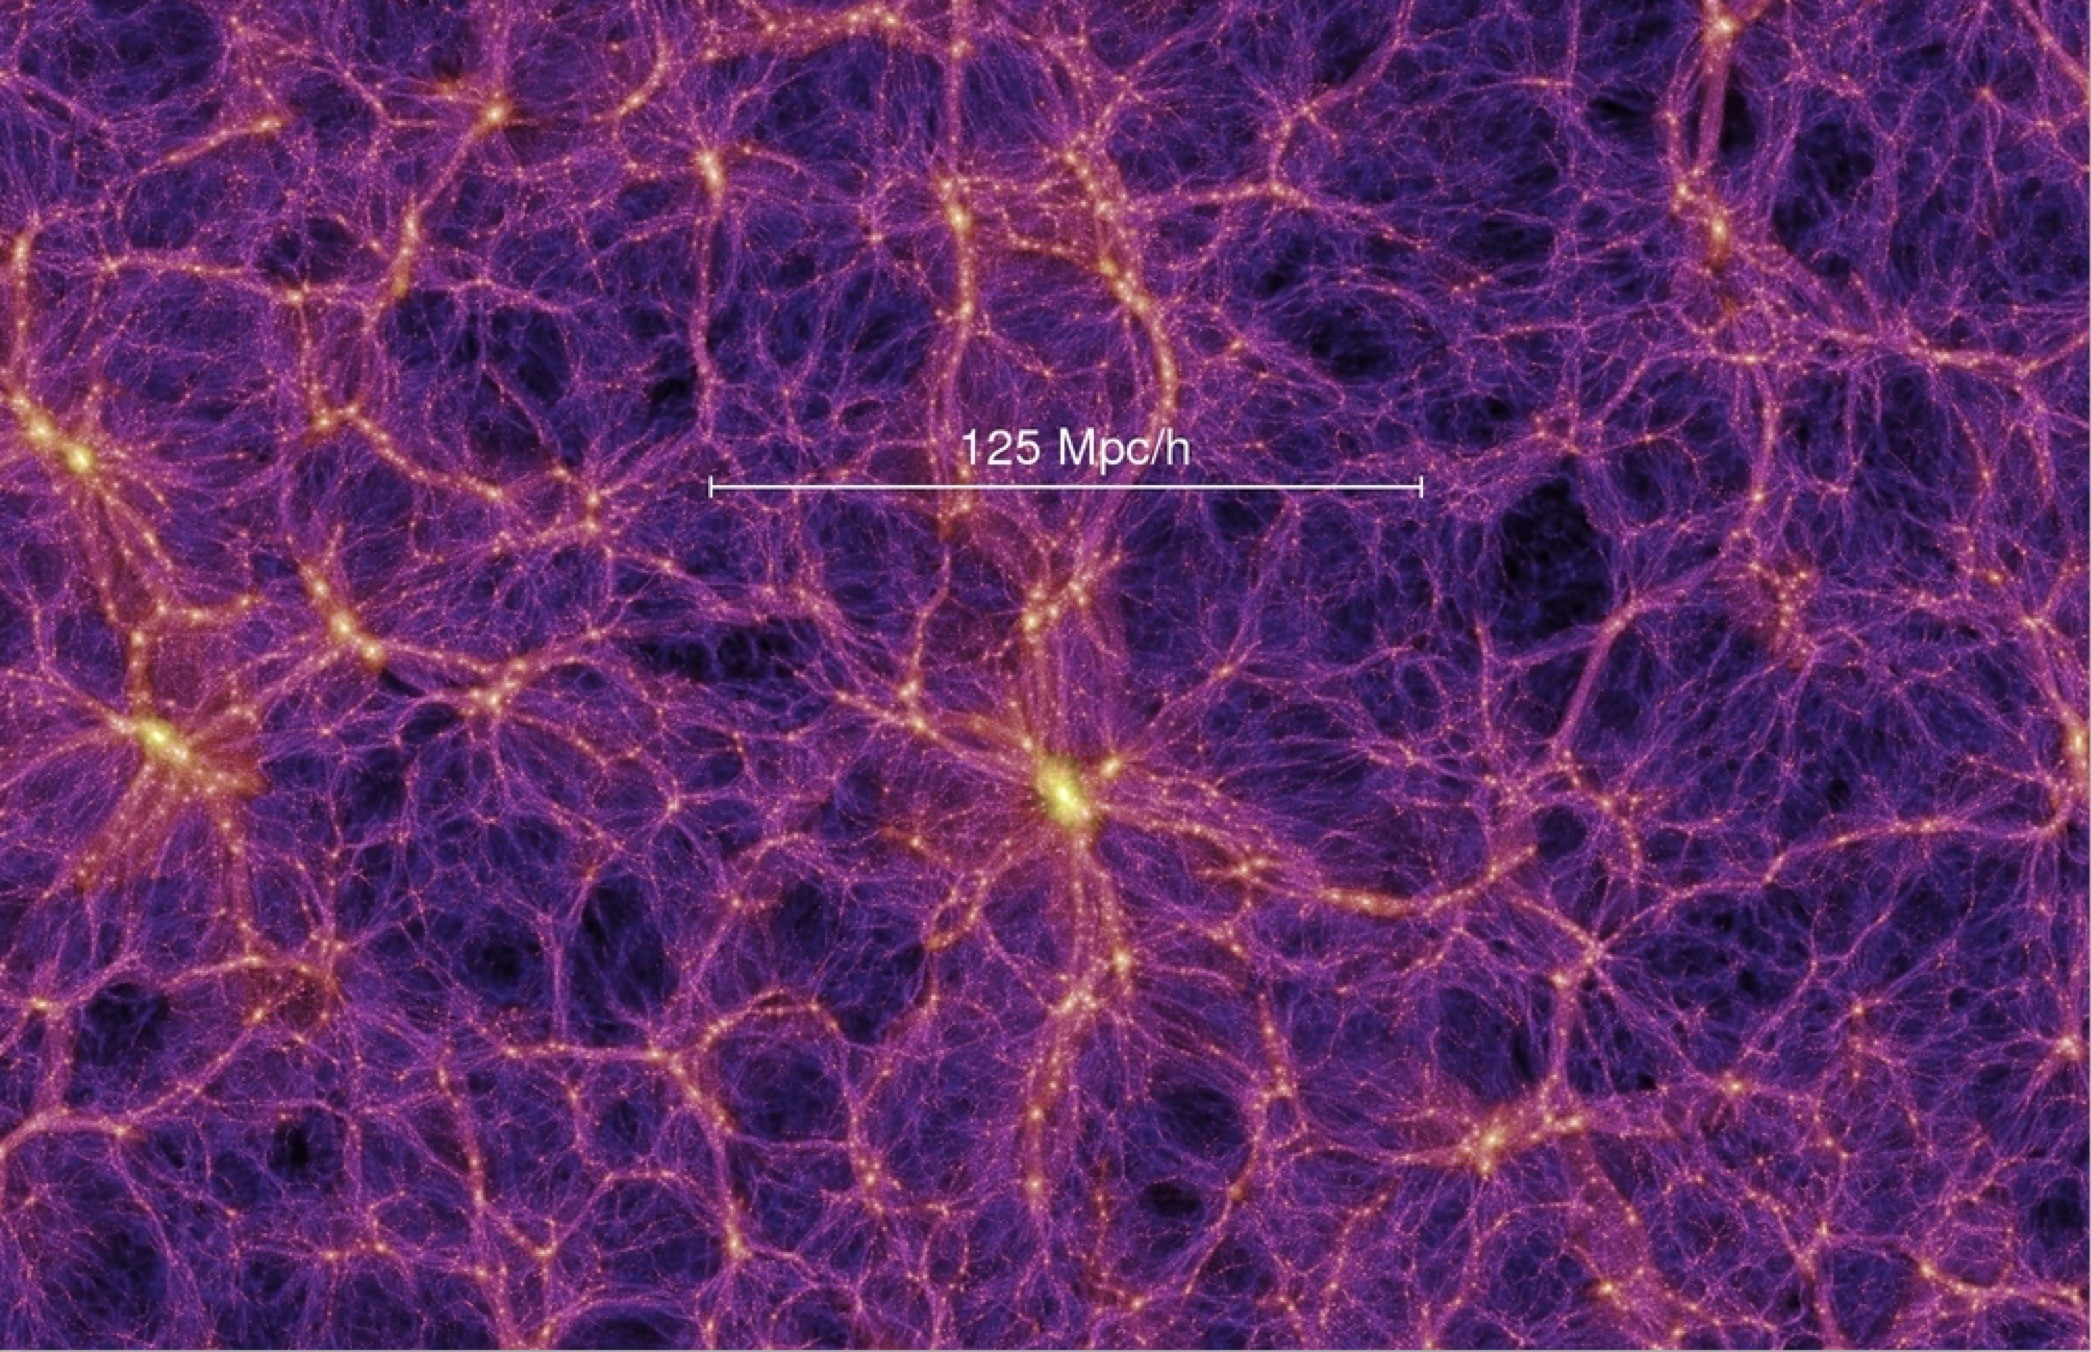
\includegraphics[width=.6\linewidth]{photo/1.jpg}
	\caption{Крупномасштабная структура Вселенной}
	\label{fig:figure1}
\end{figure}
\begin{figure}[tb]
	\centering
	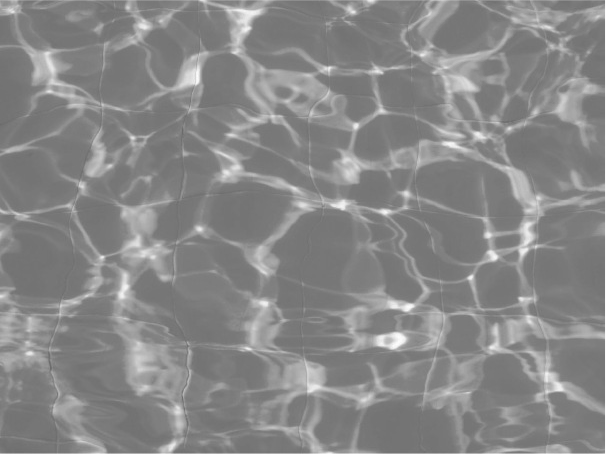
\includegraphics[width=.6\linewidth]{photo/2.png}
	\caption{Система каустик на дне бассейна}
	\label{fig:figure2}
\end{figure}
В заключение отметим, что результаты динамического моделирования в рамках приближения слипания можно посмотреть на Youtube (\textbf{The Sticky Geometry of the Cosmic Web, version 2.01})

\url{https://www.youtube.com/watch?v=wI12X2zczqI}

Результаты прямого численного моделирования (N-body simulation) можно также  посмотреть на Youtube

Двухмерный случай:

\url{https://www.youtube.com/watch?v=nHvcqV92oqY}

\url{https://www.youtube.com/watch?v=74IsySs3RGU}

Трехмерный случай

\url{https://www.youtube.com/watch?v=eDGtFRj4xXc}

\newpage
\section{Гидродинамика идеальной жидкости}

В  данном разделе мы рассмотрим законы движения и равновесия идеальной жидкости, то есть жидкости в которой не учитывается внутреннее трение, и следовательно, нет перехода механической энергии в тепловую. Будем также пренебрегать теплообменом между  различными объемами жидкости.

Это означает, что все процессы протекают при постоянной энтропии, а состояние жидкости характеризуется одной скалярной величиной --  давлением $P$. Это, конечно, идеализация, которая приводит к ряду парадоксальных результатов (например, парадокс  Даламбера-Эйлера --  сила сопротивления при равномерном движении тела в жидкости равна нулю). Тем не менее, без этой идеализации невозможно дальнейшее изучение реальных ситуаций.

\subsection{Основные уравнения гидродинамики идеальной жидкости}
Прежде чем перейти к выводу уравнений, рассмотрим два альтернативных способа описания движения жидкости. Оба они были предложены Леонардом Эйлером, но одно из них носит имя Лагранжа.
\begin{center}
{\emph{Первый способ} – \textbf{Лагранжево описание}}
\end{center}
В основу этого способа положено описание движения отдельных «жидких частиц». При этом все величины, в том числе и  координаты частицы жидкости определятся как функции времени $t$  и некоторых переменных $\xi_i(i=1,2,3)$, идентифицирующих определенную частицу («метки» частиц)
\begin{align*}
	x_i &=x_i(\xi_k,t) \\
	P &=P(\xi_k,t) \\
	\rho &=\rho(\xi_k,t) \\
	\ldots 
\end{align*}
В качестве переменных $\xi_k$ обычно используют начальные координаты частиц жидкости
\begin{align*}
	t &=t_0 \\
	\xi_i &= x_i(\xi_k,t_0)
\end{align*}

Таким образом при лагранжевом описании мы следим за определленными частицами жидкости и смотрим как изменяются во времени их координаты,  скорости, ускорения, а также давление, температура, плотность в их окрестности.

При этом скорость и ускорение частицы вычисляются как
\begin{align*}
v_{i} &=\frac{\partial x_{i}}{\partial t} \\
a_{i} &=\frac{\partial^{2} x_{i}}{\partial t^{2}} 
\end{align*}
Здесь $ \vec{v}\left(\xi_{k}, t\right) $ - скорость частицы в момент времени $t$ имела координаты $\xi_1,\xi_2,\xi_3$.

Отметим, что такому описанию соответствует способ исследования океана (реки Волги) с помощью геофизических буев с нулевой плавучестью.
\begin{figure}[H]
	\centering
	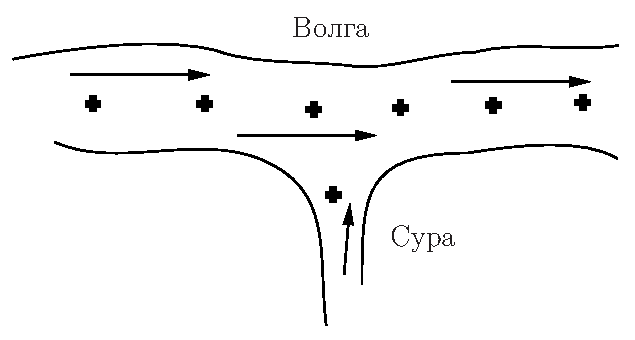
\includegraphics[scale=1]{photo/3.pdf}
	\caption{Схематичная картина Лагранжева и Эйлерова описания. \ding{58} - якорь.}
	\label{fig:figure3}
\end{figure}
\begin{center}
	{\emph{Второй способ} – \textbf{Эйлерово описание}}
\end{center}

Неподвижное пространство заполнено движущейся жидкостью. Движение жидкости будет определено если все величины характеризующую жидкость (скорость движения, давление, плотность, температура и т.д.) \textcolor{red}{будут определены}.
То есть мы следим, как меняются эти величины от точки к точке
\begin{align*} 
\vec{v} &=\vec{v}(\vec{x}, t) \\
T &=T(\vec{x}, t)
\end{align*}
Система заякоренных буев. 
В Эйлеровом описании мы не знаем что делается с отдельной частицей. При этом частные производные от скорости не являются ускорением. Так если течение стационарно и частная производная по времени  равна нулю, частицы в данной точке могут иметь ускорение. Пример – водопад.

Найдем ускорение частицы. За время $ \Delta t $ частица находящаяся в момент времени $t$ в точке с координатами $ x_{k} $ переместится в точку $ x_{k}=x_{k}+\Delta x_{k} $. Тогда для $i$-ой компоненты ускорения имеем
\begin{align*} 
\lim _{\Delta t \rightarrow 0} \frac{\Delta x_{k}}{\Delta t} &=\frac{\partial x_{k}}{\partial t}=v_{k} 
\end{align*}
\begin{align*}
a_{i} &=\lim _{\Delta t \rightarrow 0} \frac{v_{i}\left(x_{k}+\Delta x_{k}, t+\Delta t\right)-v_{i}\left(x_{k}, t\right)}{\Delta t} \\
&=\lim _{\Delta t \rightarrow 0}\frac{\left[v_{i}\left(x_{k}, t\right)+\frac{\partial v_{i}}{\partial x_{k}} \Delta x_{k}+\frac{\partial v_{i}}{\partial t}-v_{i}\left(x_{k}, t\right)\right]}{\Delta t} \\
&=\frac{\partial v_{i}}{\partial x_{k}} v_{k}+\frac{\partial v_{i}}{\partial t} \\
\end{align*}
Таким образом 
\begin{align*} 
a_{i} &=\frac{\partial v_{i}}{\partial t}+v_{k} \frac{\partial v_{i}}{\partial t}=\left(\frac{\partial}{\partial t}+v_{k} \frac{\partial}{\partial t}\right) v_{i} \\
\vec{a} &=\frac{\partial \vec{v}}{\partial t}+(\vec{v} \nabla) \vec{v}=\left(\frac{\partial}{\partial t}+(\vec{v} \nabla)\right) \vec{v}
\end{align*}

Аналогично находятся и производные от любой другой величины. Эта производная носит название субстанциональной производной.
\begin{align*} 
\frac{d}{d t}=\frac{\partial}{\partial t}+(\vec{v} \nabla)
\end{align*}
\subsection{Переход от Эйлерова описания к Лагранжеву и обратно}
Пусть известно Эйлерово поле скорости $ \vec{v}=\vec{v}(\vec{x}, t) $. Чтобы найти как двигаются Лагранжевы частицы $ \vec{x}(t, \vec{\xi}) $ нужно решить уравнение
\begin{align*} 
\frac{d \vec{x}}{d t}=\vec{v}(\vec{x}, t) \\
\vec{x}(t=0, \vec{\xi})=\vec{\xi}
\end{align*}
Как найти эйлерово поле скорости? Если нам известно поведение лагранжевых частиц $ \vec{x}(t, \vec{\xi}) $, то вначале нам нужно решить уравнение 
\begin{align*} 
\vec{x}=\vec{x}(t, \vec{\xi})
\end{align*}

Решение этого уравнения 
\begin{align*} 
\vec{\xi}=\vec{\xi}(\vec{x}, t)
\end{align*}
позволяет найти Лагранжеву частицу, которая в момент времени $t$ попала в точку $x$. Тогда эйлерово поле скорости будет равно
\begin{align*} 
\vec{v}(\vec{x}, t)=\vec{v}(t, \vec{\xi}(\vec{x}, t)
\end{align*}
\subsection{Уравнение непрерывности и закон сохранения массы}
Пусть имеется некоторый объем пространства $V$ заполненный движущейся  жидкостью. Количество жидкости (масса) в этом объеме равно:
\begin{align*} 
m=\int\limits_{V} \rho d V
\end{align*}
где $\rho$ - плотность жидкости. Жидкость может притекать и вытекать из объема. Введем элемент поверхности $ d \sigma $ и вектор $ d \vec{\sigma}=d \sigma \vec{n} $, направленный по внешней нормали к поверхности. 
\begin{figure}[H]
	\vspace{-10pt}
	\centering
	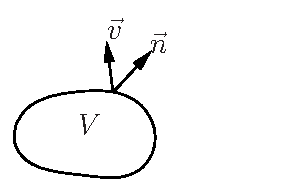
\includegraphics[scale=1]{photo/4.pdf}
	\caption{Объем, скорость и нормаль к поверхности}
	\label{fig:figure4}
\end{figure}
Поток через элемент поверхности определяется скалярным произведением:
\begin{align*}
\oint\limits_{S} \rho \vec{v} d \vec{\sigma}=\int\limits_{V} \Div(\rho \vec{v}) d V
\end{align*}


Уравнение баланса имеет вид:
\begin{align*} 
\frac{\partial}{\partial t} \int\limits_{V} \rho d V=-\oint\limits_{S} \rho \vec{v} d \vec{\sigma}
\end{align*}
Это интегральный закон сохранения массы. Если на поверхности скорость равна нулю, то масса сохраняется.

Используя формулу Остроградского-Гаусса
\begin{align*} 
\oint\limits_{S} \rho \vec{v} d \vec{\sigma}=\int\limits_{V} \operatorname{div}(\rho \vec{v}) d V
\end{align*}
получим 
\begin{align*} 
\int\limits_{V}\left[\frac{\partial \rho}{\partial t}+\Div(\rho \vec{v})\right] d V=0
\end{align*}

Так как объем произвольный, то мы получаем дифференциальный закон сохранения
\begin{align*} 
\frac{\partial \rho}{\partial t}+\Div(\rho \vec{v})=0
\end{align*}

Вектор $ \vec{j}=\rho \vec{v} $ - плотность потока массы. Используя формулу $ \nabla(a \vec{b})=\nabla a \vec{b}+a \nabla \vec{b} $, перепишем закон сохранения массы в виде:
\begin{align*} 
\frac{\partial \rho}{\partial t}+(\vec{v} \nabla) \rho+\rho \Div(\vec{v})=0 \\
\frac{d \rho}{d t}=-\rho \Div(\vec{v})=0
\end{align*}

\textbf{Несжимаемая жидкость - плотность вдоль траектории частицы не меняется.}
\begin{align*} 
\frac{d \rho}{d t}=0
\end{align*}
То есть поле скорости соленоидально $\Div\vec{v}=0$.